\documentclass[12pt]{article}
\usepackage[left=1in,right=1in,top=1in,bottom=1in]{geometry}%
\let\bibsection\relax
\usepackage{amsrefs}
\usepackage{amsmath}
\usepackage{enumerate}
\usepackage{amssymb}                
\usepackage{amsmath}                
\usepackage{amsfonts}
\usepackage{amsthm}
\usepackage{bbm}
\usepackage{float}
\usepackage{mathtools}
\usepackage{graphicx,epsfig}
\usepackage{hyperref}

\RequirePackage{xcolor}[2.11]
\colorlet{siaminlinkcolor}{green!50!black}
\colorlet{siamexlinkcolor}{red!50!black}
\colorlet{siamreviewcolor}{black!50}
\hypersetup{
  hidelinks = true,
  colorlinks = false,
  allcolors = siaminlinkcolor,
  urlcolor = siamexlinkcolor,
}

\usepackage[capitalize,nameinlink]{cleveref}
% Per SIAM Style Manual, "section" should be lowercase
\crefname{section}{section}{sections}
\crefname{subsection}{subsection}{subsections}
\Crefname{section}{Section}{Sections}
\Crefname{subsection}{Subsection}{Subsections}

% Per SIAM Style Manual, "Figure" should be spelled out in references
\Crefname{figure}{Figure}{Figures}

% Per SIAM Style Manual, don't say equation in front on an equation.
\crefformat{equation}{\textup{#2(#1)#3}}
\crefrangeformat{equation}{\textup{#3(#1)#4--#5(#2)#6}}
\crefmultiformat{equation}{\textup{#2(#1)#3}}{ and \textup{#2(#1)#3}}
{, \textup{#2(#1)#3}}{, and \textup{#2(#1)#3}}
\crefrangemultiformat{equation}{\textup{#3(#1)#4--#5(#2)#6}}%
{ and \textup{#3(#1)#4--#5(#2)#6}}{, \textup{#3(#1)#4--#5(#2)#6}}{, and \textup{#3(#1)#4--#5(#2)#6}}

% But spell it out at the beginning of a sentence.
\Crefformat{equation}{#2Equation~\textup{(#1)}#3}
\Crefrangeformat{equation}{Equations~\textup{#3(#1)#4--#5(#2)#6}}
\Crefmultiformat{equation}{Equations~\textup{#2(#1)#3}}{ and \textup{#2(#1)#3}}
{, \textup{#2(#1)#3}}{, and \textup{#2(#1)#3}}
\Crefrangemultiformat{equation}{Equations~\textup{#3(#1)#4--#5(#2)#6}}%
{ and \textup{#3(#1)#4--#5(#2)#6}}{, \textup{#3(#1)#4--#5(#2)#6}}{, and \textup{#3(#1)#4--#5(#2)#6}}

% Make number non-italic in any environment.
\crefdefaultlabelformat{#2\textup{#1}#3}

\def\noi{\noindent}
\def\T{{\mathbb T}}
\def\R{{\mathbb R}}
\def\N{{\mathbb N}}
\def\C{{\mathbb C}}
\def\Z{{\mathbb Z}}
\def\P{{\mathbb P}}
\def\E{{\mathbb E}}
\def\Q{\mathbb{Q}}
\def\ind{{\mathbb I}}

\def\calH{{\mathcal H}}
\def\calE{{\mathcal E}}
\def\calQ{{\mathcal Q}}
\def\calL{{\mathcal L}}


\DeclareMathOperator{\spn}{span}
\DeclareMathOperator{\ran}{ran}

\newtheorem{lemma}{Lemma}
\newtheorem{theorem}{Theorem}
\newtheorem{corollary}{Corollary}
\newtheorem{definition}{Definition}
\newtheorem{hypothesis}{Hypothesis}
\newtheorem{remark}{Remark}

\graphicspath{ {images/} }

\title{Multi-pulse solitary waves in fourth-order NLS equation}

\begin{document}

\maketitle

% \begin{frontmatter}
% \title{NLS4}

% \author[1]{Ross Parker}
%     \ead{ross\_parker@brown.edu}
% \author[1]{Bj\"{o}rn Sandstede}
%     \ead{bjorn\_sandstede@brown.edu}

% \address[1]{Division of Applied Mathematics, Brown University, Providence, RI 02912, USA}

% \begin{abstract}
% \end{abstract}

% \begin{keyword}
% \end{keyword}
% \end{frontmatter}

\section{Introduction}

\section{Background}

The following fourth-order generalization of the nonlinear Schr{\"o}dinger equation (NLS)
\begin{equation}\label{NLS4}
i \psi_t + \frac{\beta_4}{24}\psi_{xxxx} - \frac{\beta}{2}\psi_{xx} + \gamma |\psi|^2 \psi = 0,
\end{equation}
was recently investigated in \cite{Tam2020} in a study of the properties of solitary wave solutions under a combination of second- and fourth-order dispersion. (We use the independent variables $(t, x)$ in place of $(z, \tau)$ in \cite{Tam2020}). Ordinary NLS solitons are solutions when $\beta_2 < 0$ and $\beta_4 = 0$. Pure quartic solitons (PQSs) occur when $\beta_2 = $ and $\beta_4 < 0$, i.e. satisfy the equation
\begin{equation}\label{PQSeq}
i \psi_t + \frac{\beta_4}{24}\psi_{xxxx} + \gamma |\psi|^2 \psi = 0,
\end{equation}
By using the rescaling $\psi(x; \omega) = \sqrt{\frac{\omega}{\gamma}}\phi(\omega^{1/4}x)$, 

There has been much recent interest in PQSs due to the their discovery in experimental media by Blanco-Redondo et al. in 2016 \cite{BlancoPQS}. The existence and spectral stability of PQS solutions to \cref{NLS4} was shown in \cite{Tam2019}, and criteria for existence of 

Writing \cref{NLS4} as a system of real-valued equations in $u = (v, w)$,
\begin{align}\label{NLSsystem}
\frac{\partial}{\partial_t}
\begin{pmatrix}v \\ w \end{pmatrix}
= J \begin{pmatrix}
-\frac{\beta_4}{24} v_{xxxx} + \frac{\beta_2}{2} v_{xx} - \gamma (v^2 + w^2)v \\
-\frac{\beta_4}{24} w_{xxxx} + \frac{\beta_2}{2} w_{xx} - \gamma (v^2 + w^2)w 
\end{pmatrix}
\end{align}
where 
\[
J = \begin{pmatrix}0 & 1 \\ -1 & 0 \end{pmatrix}
\]
is the standard skew-symplectic matrix. Equation \cref{NLSsystem} can be written in Hamiltonian form as 
\begin{equation}\label{NLSHam}
\frac{\partial u}{\partial t} = J \calE'(u(t))
\end{equation}
where the energy $\calE$ is given by
\begin{equation}\label{defH}
\calE(v, w) = \frac{1}{2} \int_{\infty}^\infty \left( \frac{\beta_4}{24}\left( v_{xx}^2 + w_{xx}^2 \right) + \frac{\beta_2}{2}\left( v_{x}^2 + w_{x}^2 \right) + \gamma \left(v^2 + w^2 \right)^2 \right) dx
\end{equation}
The energy $\mathcal{E}$ is invariant under the standard rotation group $T(\theta)$, given by
\begin{equation}\label{Ttheta}
T(\theta) = \begin{pmatrix}
\cos(\theta) & -\sin(\theta) \\
\sin(\theta)& \cos(\theta)
\end{pmatrix},
\end{equation}
The corresponding conserved quantity, often called the charge \cite[Section 6.C]{Grillakis1987}, is given by
\begin{equation}\label{defQ}
\mathcal{Q}(v, w) = -\frac{1}{2} \int_{\infty}^\infty \left( v^2 + w^2\right) dx.
\end{equation}
Standing waves are solutions of the form $T(\omega t) u$, where $u$ is independent of $t$. A standing wave solution satisfies the standing wave equation $\calE'(u) - w \calQ'(u) = 0$ \cite[2.15]{Grillakis1987}. Since $\calQ'(u) = -u$, the standing wave equation is
\begin{equation}\label{standingwaveeq}
\calE'(u) + w u = 0
\end{equation}

Suppose that for all $\omega \in (\omega_1, \omega_2)$ there exists a bound state solution $u(x; \omega)$ to \cref{standingwaveeq}, and that the mapping $\omega \mapsto u(x; \omega)$ is $C^1$ \cite[Assumption 2]{Grillakis1987}. Define the scalar
\begin{equation}
d(\omega) = \calE(u(\omega)) - \omega\calQ(u(\omega)).
\end{equation}
By \cite[(2.21)]{Grillakis1987},
\begin{align}\label{ddoubleprime}
d''(\omega) = \langle \calQ'(u(x; \omega)), \partial_\omega u(x; \omega) \rangle
= \int_{-\infty}^\infty u(x) \partial_\omega u(x) dx
\end{align}
By \cite[Theorem 3.5]{Grillakis1987}, the standing wave $u(x; \omega)$ is orbitally stable if $d''(\omega) > 0$. This quantity is easy to compute numerically.

Let $\phi$ be a real-valued standing wave solution to \cref{standingwaveeq}. The linearization of the PDE \cref{NLSsystem} about $\phi$ is the linear operator $\calL(\phi)$
\begin{align}\label{defLphi}
\calL(\phi) = 
\begin{pmatrix}
0 & \calL^-(\phi) \\
-\calL^+(\phi) & 0
\end{pmatrix},
\end{align}
where
\begin{align*}
\calL^-(\phi) &= -\frac{\beta_4}{24} \partial_{xxxx} + \frac{\beta_2}{2} \partial_{xx} + \omega - \gamma \phi^2 \\
\calL^+(\phi) &= -\frac{\beta_4}{24} \partial_{xxxx} + \frac{\beta_2}{2} \partial_{xx} + \omega - 3 \gamma \phi^2
\end{align*}
It is straightforward to verify that 
\begin{align*}
\calL^-(\phi) \phi &= 0 \\
\calL^+(\phi) \partial_x \phi &= 0 \\
\calL^+(\phi)(-\partial_\omega \phi) &= \phi
\end{align*}
Furthermore, since $\calL^-$ is self-adjoint and $\phi' \perp \ker \calL^-$, there exists $z$ such that $\calL^- z = u'$. For ordinary NLS ($\beta_4 = 0, \beta_2 \neq 0$), $z = \frac{1}{2 \beta_2} x \phi$. For the general case, $z$ exists and is easy to compute numerically, but I am not sure there is a nice formula for it.

Putting all of this together, $\calL(\phi)$ has a kernel with (at least) algebraic multiplicity 4 and geometric multiplicity 2, i.e.
\begin{align*}
\calL(\phi)\begin{pmatrix}0 \\ \phi \end{pmatrix} &= 0, 
\calL(\phi)\begin{pmatrix} \partial_\omega \phi \\ 0 \end{pmatrix} = \begin{pmatrix}0 \\ \phi \end{pmatrix} \\
\calL(\phi)\begin{pmatrix}\partial_x\phi \\ 0 \end{pmatrix} &= 0, 
\calL(\phi)\begin{pmatrix} 0 \\ z \end{pmatrix} = \begin{pmatrix}\partial_x\phi \\ 0 \end{pmatrix} 
\end{align*}

Now let $\phi$ be an exponentially localized bound state solution. For the essential spectrum, which is independent of $\phi$ and only depends on the background state, the linear operator $\calL(\phi)$ is exponentially asymptotic to $\calL(0)$, given by
\begin{align}\label{defL0}
\calL(0) = 
\begin{pmatrix}
0 & \calL_0 \\
-\calL_0 & 0
\end{pmatrix},
\calL_0 = -\frac{\beta_4}{24} \partial_{xxxx} + \frac{\beta_2}{2} \partial_{xx} + \omega
\end{align}.
Thus the eigenvalue problem $\calL(0) v = \lambda v$ is equivalent to $(\calL_0 + \lambda^2)p = 0$. By \cite[Theorem 3.1.13]{Kapitula2013}, the essential spectrum is given by the curves
\begin{align*}
\left[ -\frac{\beta_4}{24} (ik)^4 + \frac{\beta_2}{2}(ik)^2 + \omega \right]^2 + \lambda^2 &= 0 && k \in \R.
\end{align*}
As long as $\beta_2, \beta_4 < 0$ (and $\omega > 0$), the essential spectrum is purely imaginary, and the curves are
\begin{align*}
\lambda = \pm i \left( -\frac{\beta_4}{24}k^4 - \frac{\beta_2}{2}k^2 + \omega \right).
\end{align*}
For $\beta_4, \beta_2 \leq 0$, the essential spectrum is the subset of the imaginary axis given by
\begin{equation}\label{PQSessspec}
\sigma_{ess} = \{ k i : |k| \geq \omega \},
\end{equation}
which is bounded away from the origin and does not depend on $\beta_2,\beta_4$. In particular, this is the case for pure quartic solitary waves. For $\beta_4 < 0, \beta_2 > 0$, the essential spectrum is the subset of the imaginary axis 
\begin{equation}
\sigma_{ess} = \{ k i : |k| \geq (\omega - \omega_c) \},
\end{equation}
which does depend on $\beta_2,\beta_4$, but is bounded away from the origin for $\omega > \omega_c$, where $\omega_c$ is defined below in \cref{omegac}.

\section{Existence of multi-pulses}

Real-valued, standing wave solutions to \cref{standingwaveeq} satisfy the 4th order ODE
\begin{equation}\label{NLS4real}
-\frac{\beta_4}{24} u_{xxxx} + \frac{\beta_2}{2} u_{xx} - \gamma u^3 + \omega u = 0
\end{equation}
For ordinary NLS ($\beta_4 = 0$), an exact solitary wave solution is known. For certain values of $\beta_2, \beta_4 < 0$ (i.e. those for which the solitary wave does not have an oscillating tail), an exact solitary wave solution is also known \cite[(5)]{Tam2020} (from Karlsson and Hook, 1994). For $\beta_4 = -1$, \cite[Figure 4(a)]{Tam2020} depicts regions in the $(\beta_2, \omega)$ plane where solitary wave solutions have been shown to exist (numerically, at least). For our purposes, we are interested only in solitary waves with oscillating tails. For now, we assume all such solutions exist, although it may be possible to show that.

Assume that $\beta_4 \neq 0$, so that \cref{NLS4real} does not reduce to the ordinary NLS equation. We rewrite equation \cref{NLS4real} by letting $U = (u_1, u_2, u_3, u_4) = (u, \partial_x u, \partial_x^2 u, \frac{\beta_4}{24} \partial_x^3 u)$ to get the first order system
\begin{equation}\label{Fsystem}
U' = F(U) = \begin{pmatrix}
u_2 \\ u_3 \\ \frac{24}{\beta_4} u_4 \\ \omega u_1 - \gamma u_1^3.
\end{pmatrix}
\end{equation}
Equation \cref{Fsystem} has a conserved quantity
\begin{equation}\label{FsystemH}
H(u_1, u_2, u_3, u_4) = -u_4 u_2 - \frac{1}{2} u_3^2 + \frac{\beta_2}{4}u_2^2 - \frac{\gamma}{4} u_1^4 + \frac{1}{2}\omega u_1,
\end{equation}
which we obtain by multiplying \cref{NLS4real} by $u_x$ and integrating once, where the first term on the RHS is also integrated by parts. $F(0) = 0$, and the characteristic polynomial of $DF(0)$ is
\[
p(t) = t^4 - 12\frac{\beta_2}{\beta_4} t^2 - \frac{24}{\beta_4}\omega,
\]
which has a quartet of complex eigenvalues $\pm a \pm b i$ when $3 \beta_2^2 + 2 \omega \beta_4 < 0$. For the case of $\beta_4 < 0$ (which is the one we are interested in), this is equivalent to $\omega > \omega_c$ \cite[(11)]{Tam2020}, where
\begin{equation}\label{omegac}
\omega_c = \frac{3}{2} \frac{\beta_2^2}{|\beta_4|}.
\end{equation}
Note that for the pure quartic equation, $\omega_c = 0$. Thus whenever $\omega > \omega_c$, 0 is a hyperbolic equilibrium of \cref{Fsystem} with two-dimensional stable and unstable manifolds. A primary pulse solution is a homoclinic orbit connecting this equilibrium point to itself, and corresponds to an exponentially localized solitary wave solution of \cref{NLS4real}. For $\omega > \omega_c$, the localized pulse solution corresponding to this homoclinic orbit will have exponentially decaying, oscillatory tails.

For fixed $\omega > \omega_c$, we assume the primary pulse solution $U(x) = (\phi_x, \partial_x \phi(x), \partial_x^2 \phi(x), \frac{\beta_4}{24} \partial_x^3 \phi(x))$ exists. The first component $\phi(x)$ is the corresponding solitary wave, which is the first component of $U(x)$. We assume in addition that $\phi(x)$ is orbitally stable, i.e. $d''(\omega) > 0$. Since \cref{NLSsystem} is Hamiltonian, the immediately implies that all spectrum for the linearization about the primary pulse is purely imaginary.

We have the following result concerning the existence of multi-pulse solutions, which follows immediately from \cite[Theorem~3.6]{SandstedeStrut}. The only difference is that the multi-pulse can be constructed using ``up'' and ``down'' copies of the primary pulse, so that neighboring pulses are either in phase or out of phase. This should be a straightforward adaptation.

\begin{theorem}\label{theorem:multiexist}
Assume appropriate hypotheses. Fix $\omega > \omega_c$, and let $\pm a \pm bi$ be the eigenvalues of $DF(0)$. Let $U(x)$ be an exponentially localized solution to \cref{Fsystem}. Then for any 
\begin{itemize}
\item $n \geq 2$
\item Sequence of nonnegative integers $\{ k_1, \dots, k_{n-1} \}$ with at least one of the $k_j \in \{0, 1 \}$.
\item Sequence of phase parameters $\{ \theta_1, \dots, \theta_{n-1} \} \in \{0, \pi \}^{n-1}$, which represent the phase difference between adjacent copies of the primary pulse. 
\end{itemize}
there exists a nonnegative integer $m_0$ such that for any integer $m$ with $m \geq m_0$, there exists a unique $n-$modal solution $U_n(x)$ to \cref{Fsystem} which is of the form
  \begin{equation}\label{qn}
  U_n(x) = \sum_{j = 1}^{n} e^{i \phi_n } U^j(x) + r(x),
  \end{equation}
  where each $U^j(x)$ is a translate of the primary pulse $U(x)$, and the phase of each translate $U^j(x)$ is
  \begin{equation}\label{phin}
  \phi_1 = 0, \quad \phi_n = \sum_{j=1}^{n-1} \theta_j, 
  \end{equation}
  Uniqueness is up to translation and multiplication by $T(\theta)$. The distance between the peaks of $U^j$ and $U^{j+1}$ is $2 X_j$, where
  \begin{equation*}
  X_j \approx \frac{\pi}{b}(2 m + k_j) + \tilde{X},
  \end{equation*}
  and $\tilde{X}$ is a constant. The remainder term $r(x)$ satisfies
  \begin{equation}\label{rbound}
  \|r\|_\infty \leq C e^{-a X_{\mathrm{min}}},
  \end{equation}
  where $X_{\mathrm{min}} = \min\{X_1, \dots, X_{n-1}\}$. This bound holds for all derivatives with respect to $x$.
\end{theorem}

\section{Spectrum of primary pulse}

For pure quartic solitary waves, the essential spectrum is given by \cref{PQSessspec}, which depends only on $\omega$ and is bounded away from the origin for $\omega > 0$. The boundary of the essential spectrum is at $\pm \omega i$. There are two eigenvalues at 0 resulting from translation invariance and phase invariance. There is an additional pair of eigenvalues at $\pm 0.9972 \omega i$ \cite{Tam2019} (independent of $\beta_4$) which corresponds to an internal mode of the pure quartic solitary wave. For $\beta_2 \neq 0$ (non-pure quartic solitary waves), there can be multiple pairs of internal mode eigenvalues (an example of two pairs internal mode eigenvalues is in \cite[Figure 9]{Tam2020}, which is the case $\beta_4 = -1, \beta_2 = 0.7$).

\section{Spectrum of multi-pulses}

For each $n-$pulse $\phi_n$, we can compute the spectrum of the linearized operator $\calL(\phi_n)$. Roughly speaking, since there are two eigenfunctions in the kernel of the primary pulse $\calL(\phi)$, each additional pulse in $\phi_n$ will result in four additional eigenvalues near 0 which come from nonlinear interactions between the tails of neighboring pulses in the multi-pulse structure. We call these interaction eigenvalues. To do this, we write the eigenvalue problem $\calL(\phi)u \lambda u$ as the first order system
\begin{equation}
\begin{pmatrix}v \\ w\end{pmatrix}' =
\begin{pmatrix}K_+(\phi) & 0 \\ 0 & K_-(\phi) \end{pmatrix}
\begin{pmatrix}v \\ w\end{pmatrix}
+ \lambda \begin{pmatrix}0 & B \\ -B & 0\end{pmatrix}
\begin{pmatrix}v \\ w\end{pmatrix},
\end{equation}
where
\begin{align*}
K^-(\phi) = \begin{pmatrix}
0 & 1 & 0 & 0 \\
0 & 0 & 1 & 0 \\
0 & 0 & 0 & \frac{24}{\beta_4} \\
\omega - \gamma \phi^2 & 0 & \frac{\beta_2}{2} & 0
\end{pmatrix},
K^+(\phi) = \begin{pmatrix}
0 & 1 & 0 & 0 \\
0 & 0 & 1 & 0 \\
0 & 0 & 0 & \frac{24}{\beta_4} \\
\omega - 3 \gamma \phi^2 & 0 & \frac{\beta_2}{2} & 0
\end{pmatrix},
B = \begin{pmatrix}
0 & 0 & 0 & 0 \\
0 & 0 & 0 & 0 \\
0 & 0 & 0 & 0 \\
1 & 0 & 0 & 0
\end{pmatrix}
\end{align*}
The associated variational equation and adjoint variational equation are
\begin{align}
\begin{pmatrix}v \\ w\end{pmatrix}' &=
\begin{pmatrix}K_+(\phi) & 0 \\ 0 & K_-(\phi) \end{pmatrix}
\begin{pmatrix}v \\ w\end{pmatrix} \label{vareq} \\
\begin{pmatrix}\tilde{v} \\ \tilde{w}\end{pmatrix}' &=
-\begin{pmatrix}K_+(\phi)^T & 0 \\ 0 & K_-(\phi)^T \end{pmatrix}
\begin{pmatrix}\tilde{v} \\ \tilde{w}\end{pmatrix} \label{adjvareq}
\end{align}
The variational equation \cref{vareq} has two linearly independent, exponentially decaying solutions $V_+(x) = U'(x)$ and $V_-(x) = U(x)$, where $U(x) = (\phi_x, \partial_x \phi(x), \partial_x^2 \phi(x), \frac{\beta_4}{24} \partial_x^3 \phi(x))$ is the primary pulse. Corresponding to these are two linearly independent, exponentially decaying solutions $\Psi_+(x)$ and $\Psi_-(x)$ to the adjoint variational equation \cref{vareq}. 

At this point, we can (and eventually will!) state a theorem which will give us formulas for the interaction eigenvalues. This is analogous to \cite[Theorem 2]{Sandstede1998}, and the proof is a straightforward adaptation of that theorem, with the only change being a different ansatz in place of \cite[(3.5)]{Sandstede1998}. For the present, we will just give the formulas for the interaction eigenvalues for the 2-pulse.

Let $U_2(x)$ be a 2-pulse constructed using \cref{theorem:multiexist} with pulse distance $X$ and phase difference $\theta$. Define the two Melnikov integrals
\begin{align*}
M_- &= \int_{-\infty}^\infty q(x) \partial_\omega q(x) dx \\
M_+ &= \int_{-\infty}^\infty \partial_x (x) z(x) dx,
\end{align*}
where we note that $M_- = d''(\omega)$, the stability criterion from \cite{Grillakis1987}. We are assuming that $M_- > 0$. Let 
\begin{align*}
a_- &= \langle \Psi_-(-X), V_-(X) \rangle \\
a_+ &= \langle \Psi_+(-X), V_+(X) \rangle 
\end{align*}
Then, to leading order, the four interaction eigenvalues for a 2-pulse are given by
\begin{equation}\label{inteigpred}
\begin{aligned}
\lambda_- &= \pm \sqrt{ \frac{2 a_-}{M_-} \cos(\theta) }\\
\lambda_+ &= \pm \sqrt{ \frac{-2 a_+}{M_+} \cos(\theta) }
\end{aligned}
\end{equation}
We should be able to prove that $a_i$ and $a_+$ have the same sign (numerics confirms this), so under the assumption that $M_-$ and $M_+$ are both positive, this will always give us a pair of imaginary eigenvalues and a pair of real eigenvalues, so the double pulse is unstable for both in-phase and out-of-phase configurations.

In addition, the internal mode eigenvalues of the primary pulse will duplicate as pulses are added to the multi-pulse structure. For example, for the pure quartic solitary wave, we expect that the 2-pulse will have two pairs of internal mode eigenvalues. This will not affect stability, since we have shown there is a positive, real eigenvalue.

\section{Numerical Results}

To construct the primary pulse solution $\phi(x)$, we start with the known solitary wave solution for NLS and gradually modify the parameters $\beta_2$ and $\beta_4$, solving for the new solitary wave solution at each step using a Newton conjugate-gradient method \cite[Chapter 7.2.4]{YangCh7} implemented in MATLAB. To obtain the pure quartic solitary wave (\cref{fig:PQS} for $\beta_4 = -1$, we perform this procedure along the line segment connecting $(\beta_2, \beta_4) = (-2, 0)$ and $(\beta_2, \beta_4) = (0, -1)$. Spatial discretization is a uniform grid with $N = 1024$ grid points, and we use periodic boundary conditions. The spectrum of the primary pulse solution is shown in \cref{fig:PQSspec}.

\begin{figure}[H]
\centering
\begin{tabular}{cc}
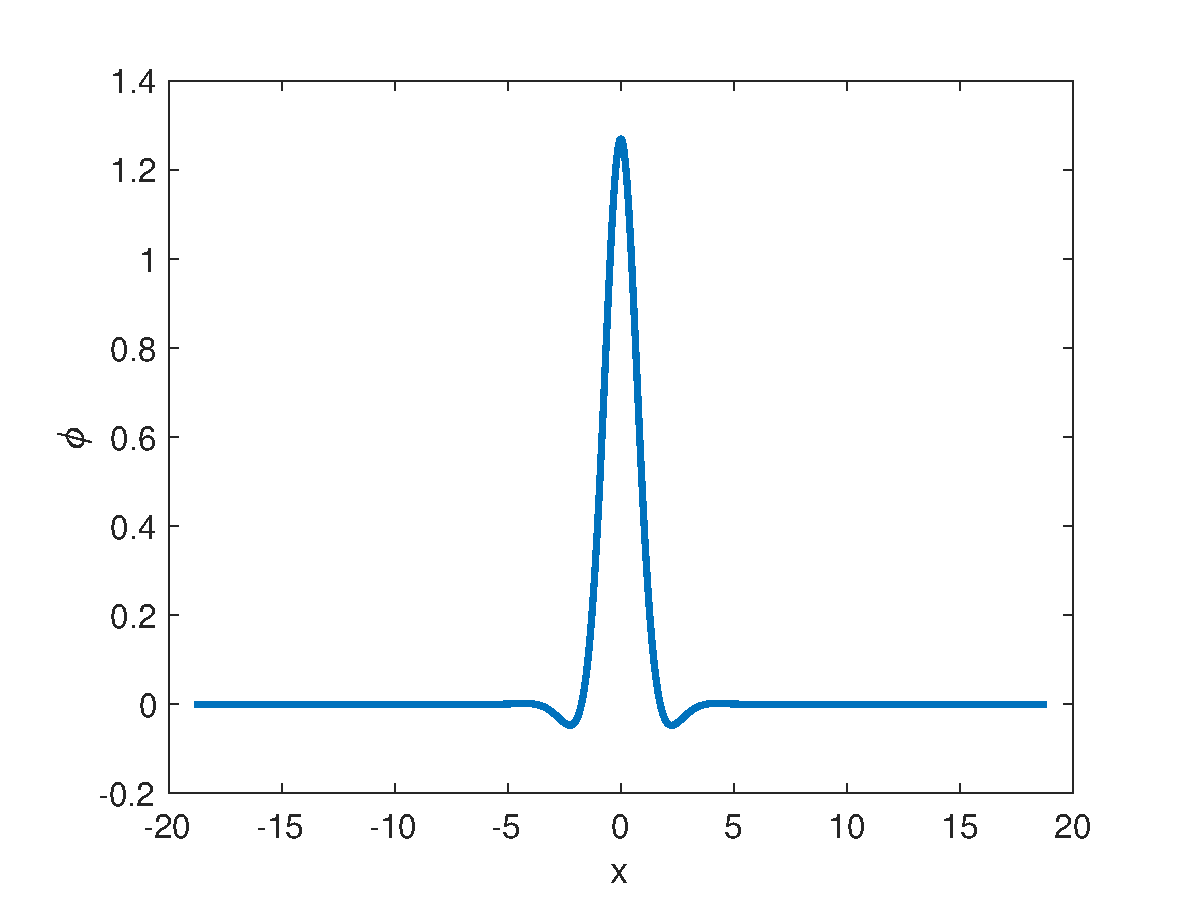
\includegraphics[width=8cm]{images/PQS1.eps} &
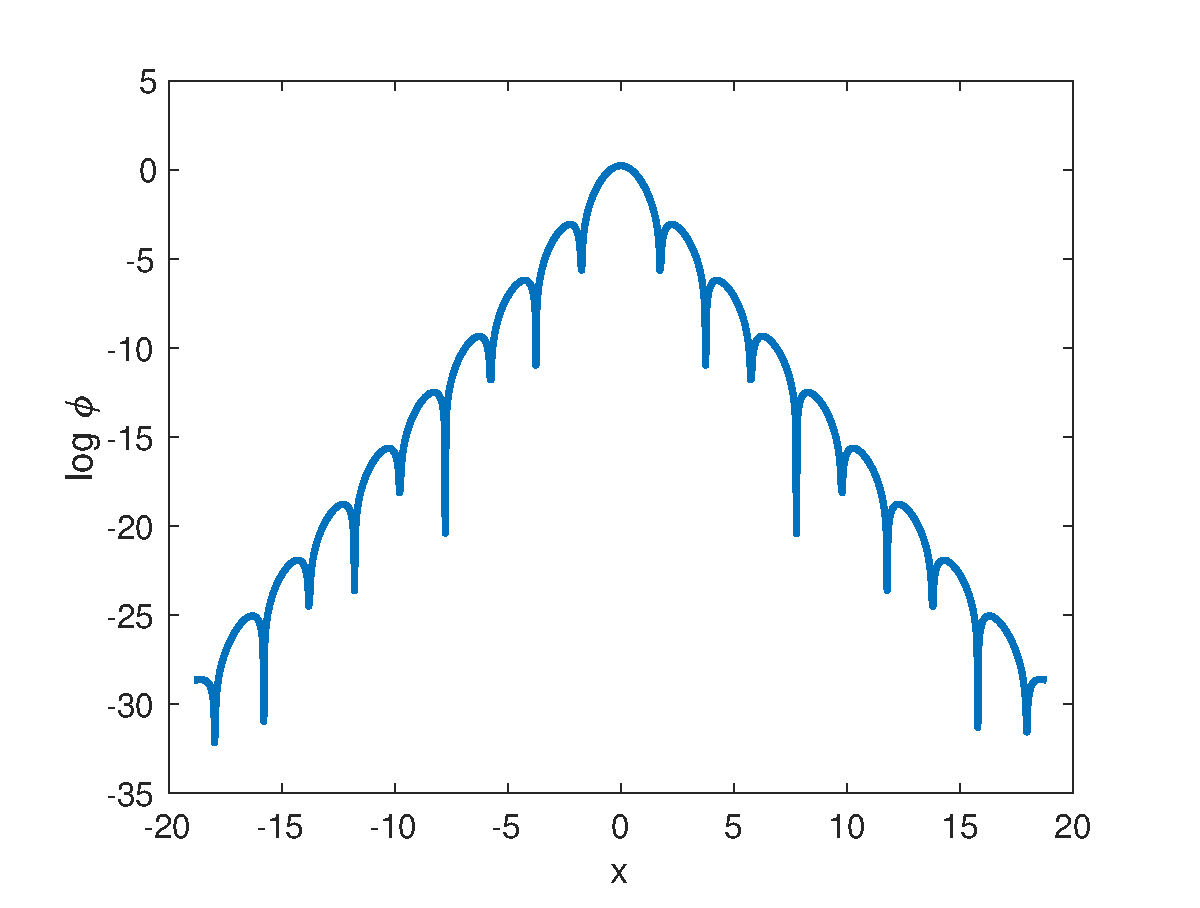
\includegraphics[width=8cm]{images/PQS1log.eps}
\end{tabular}
\caption{Pure quartic solitary wave solution $\phi(x)$ to \cref{NLS4real} with $\beta_2 = 0$, $\beta_4 = -1$, $\omega = 1$. (left panel). Plot of $\log \phi(x)$ vs $x$ (right panel) showing exponentially-decaying oscillatory tails. }
\label{fig:PQS}
\end{figure} 

\begin{figure}[H]
\centering
\begin{tabular}{cc}
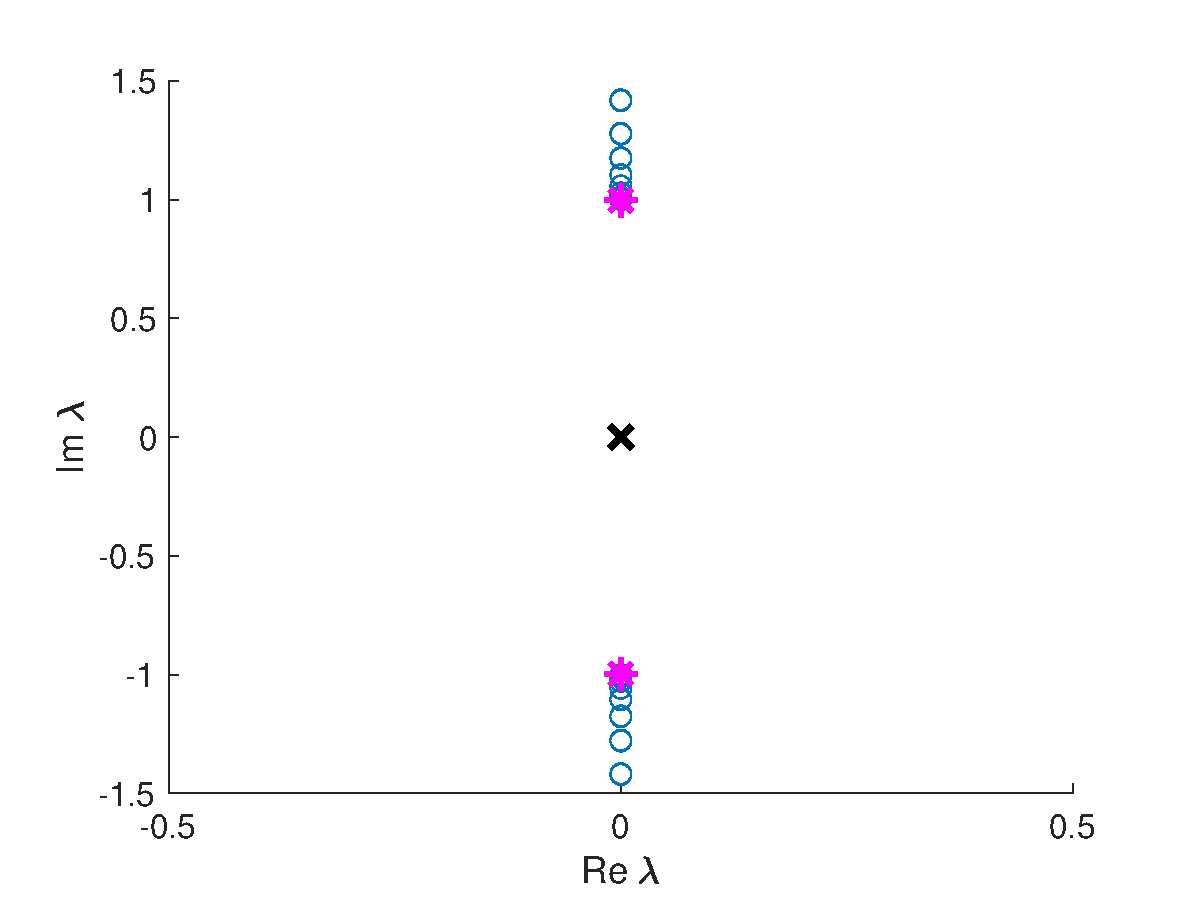
\includegraphics[width=8cm]{images/PQSspec.eps} &
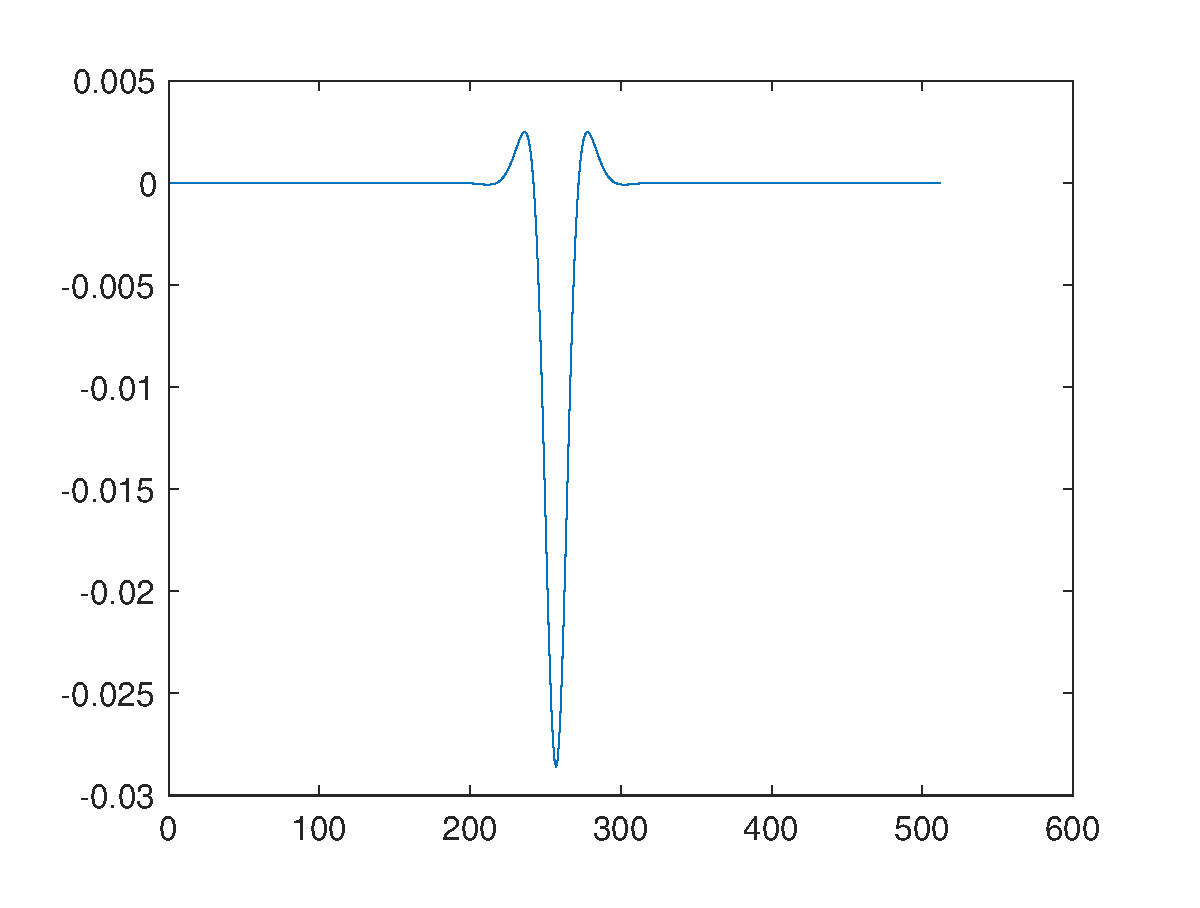
\includegraphics[width=8cm]{images/PQSinternalmode.eps}
\end{tabular}
\caption{Spectrum of pure quartic solitary wave (left panel), $\beta_2 = 0$, $\beta_4 = -1$, $\omega = 1$. Kernel eigenvalues in black, internal mode eigenvalues in red. Eigenvalues in blue correspond to the discrete essential spectrum. Eigenfunction corresponding to internal mode eigenvalues (right panel).}
\label{fig:PQSspec}
\end{figure} 

For the single pulse solitary wave solutions, we can compute the stability criterion \cref{ddoubleprime} from \cite{Grillakis1987}. In all cases we tried, $d''(\omega) > 0$ (for example for $\beta_4 = -1, \beta_2 = 0, \omega = 1$, $d''(\omega) = 0.7291$), thus the primary pulse solution is orbitally stable. (This is a much stronger result than what was done in \cite{Tam2019,Tam2020}, where they computed the spectrum numerically and found that it is purely imaginary). 

To construct double pulses, we glue together two copies of the primary pulse at the pulse distances predicted by \cref{theorem:multiexist} and solve for the double pulse solution using the same Newton conjugate-gradient method. The first eight double pulse solutions are shown in \cref{fig:doublepulses}. Arbitrary multi-pulses can similarly be constructed.

\begin{figure}[H]
\centering
\begin{tabular}{cc}
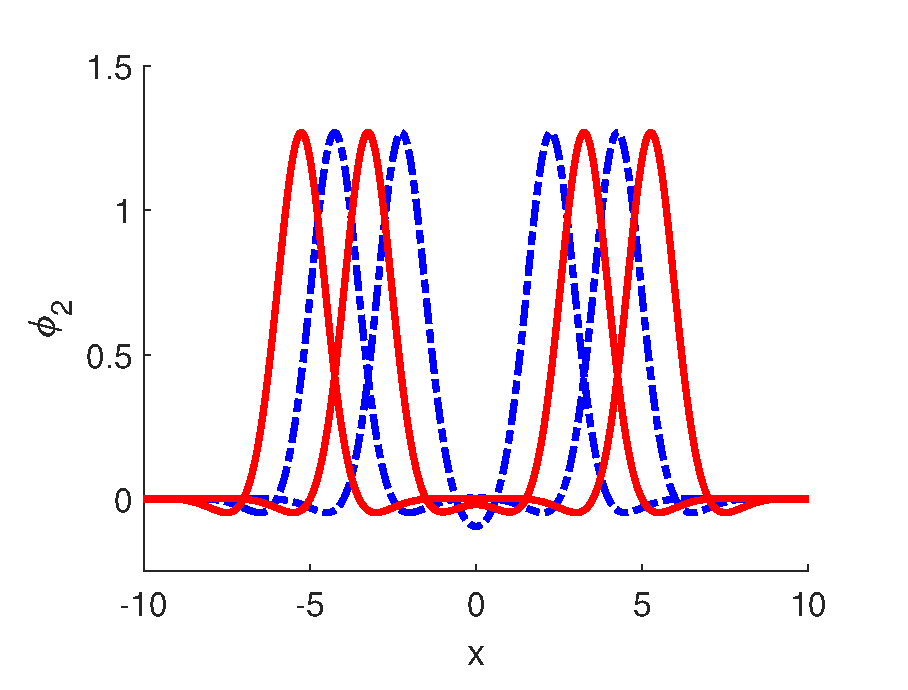
\includegraphics[width=8cm]{images/DPplus.eps} &
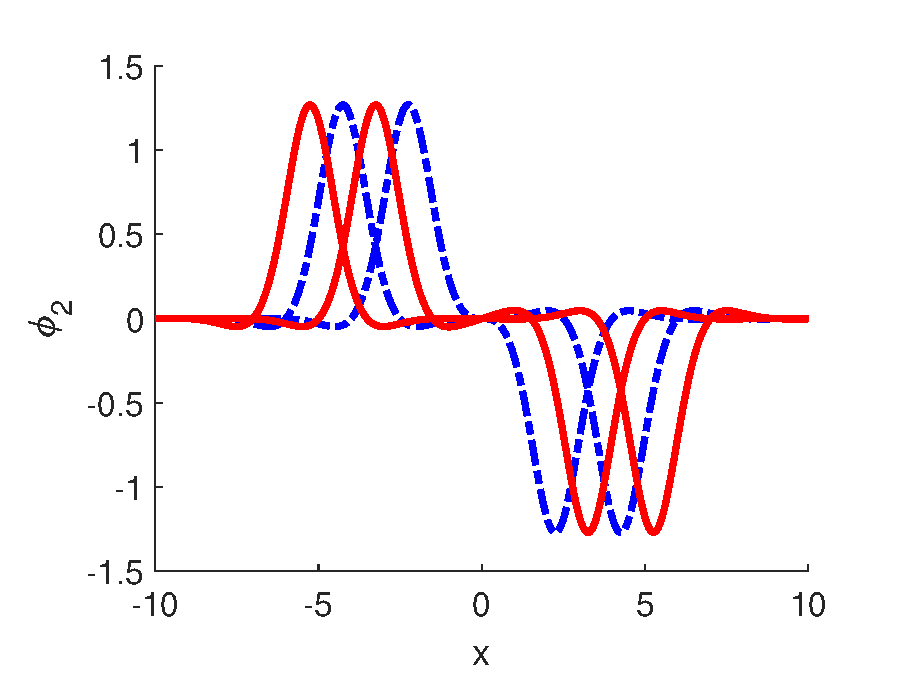
\includegraphics[width=8cm]{images/DPminus.eps}
\end{tabular}
\caption{First eight double pulse solutions $\phi_2(x)$ constructed from two pure quartic solitary wave solution $\phi(x)$ to \cref{NLS4real} with $\beta_2 = 0$, $\beta_4 = -1$, $\omega = 1$. In-phase double pulses (left panel), opposite phase double pulses (right panel). }
\label{fig:doublepulses}
\end{figure} 

To determine the spectrum of the linearization about the double pulse solutions, we construct the linear operator $\calL(\phi_2)$ using Fourier spectral differentiation matrices and compute the eigenvalues using Matlab's eigenvalue solver \texttt{eig}. In all cases, there is a pair of purely imaginary interaction eigenvalues and a pair of real interaction eigenvalues, thus the double pulses are all unstable (\cref{fig:doublespec}). There is also a duplication of the internal mode eigenvalues (\cref{fig:doubleinternalmode}). Since in all cases there is an eigenvalue with positive real part, the duplication of internal mode eigenvalues does not affect stability. 

\begin{figure}[H]
\centering
\begin{tabular}{cc}
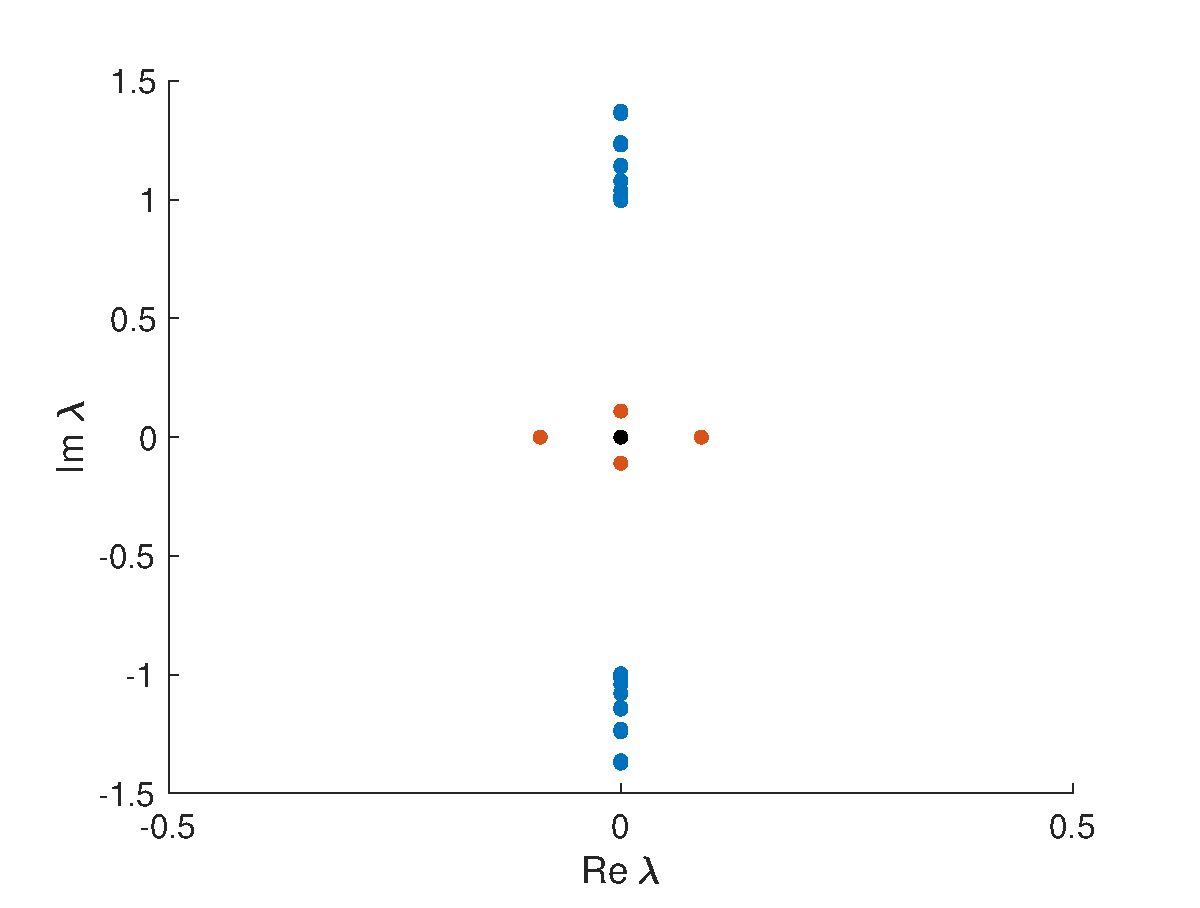
\includegraphics[width=8cm]{images/inteigsDP1plus.eps} &
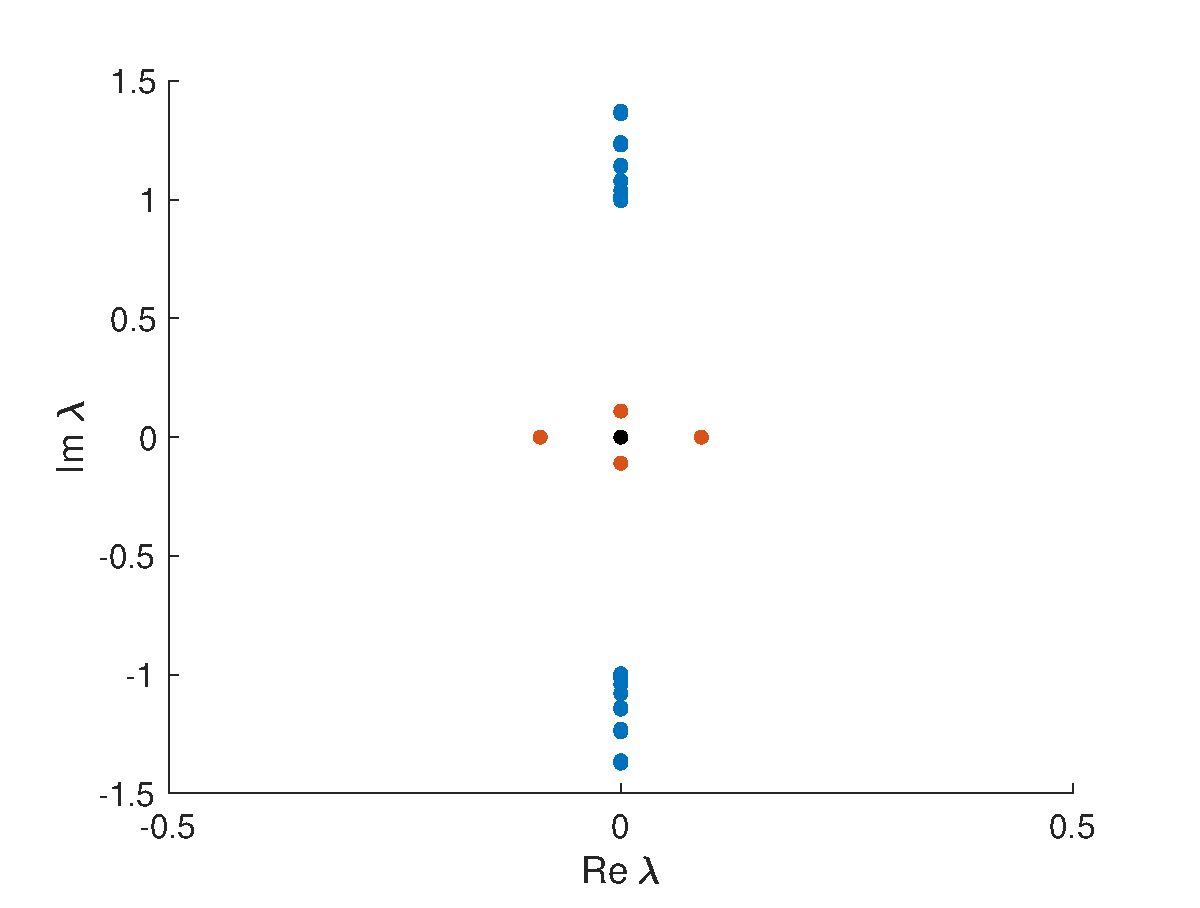
\includegraphics[width=8cm]{images/inteigsDP1plus.eps}
\end{tabular}
\caption{Eigenvalues for first in-phase double pulse (left panel) and first out-of-phase double pulse (right panel). Interaction eigenvalues shown in red, and kernel eigenvalues in black. Eigenvalues in blue correspond to the discrete essential spectrum; as expected, these eigenvalues are on the imaginary axis and have magnitude $|\lambda| \geq \omega$. Internal mode eigenvalues are not shown. $\beta_2 = 0$, $\beta_4 = -1$, $\omega = 1$.}
\label{fig:doublespec}
\end{figure} 

\begin{figure}[H]
\centering
\begin{tabular}{c}
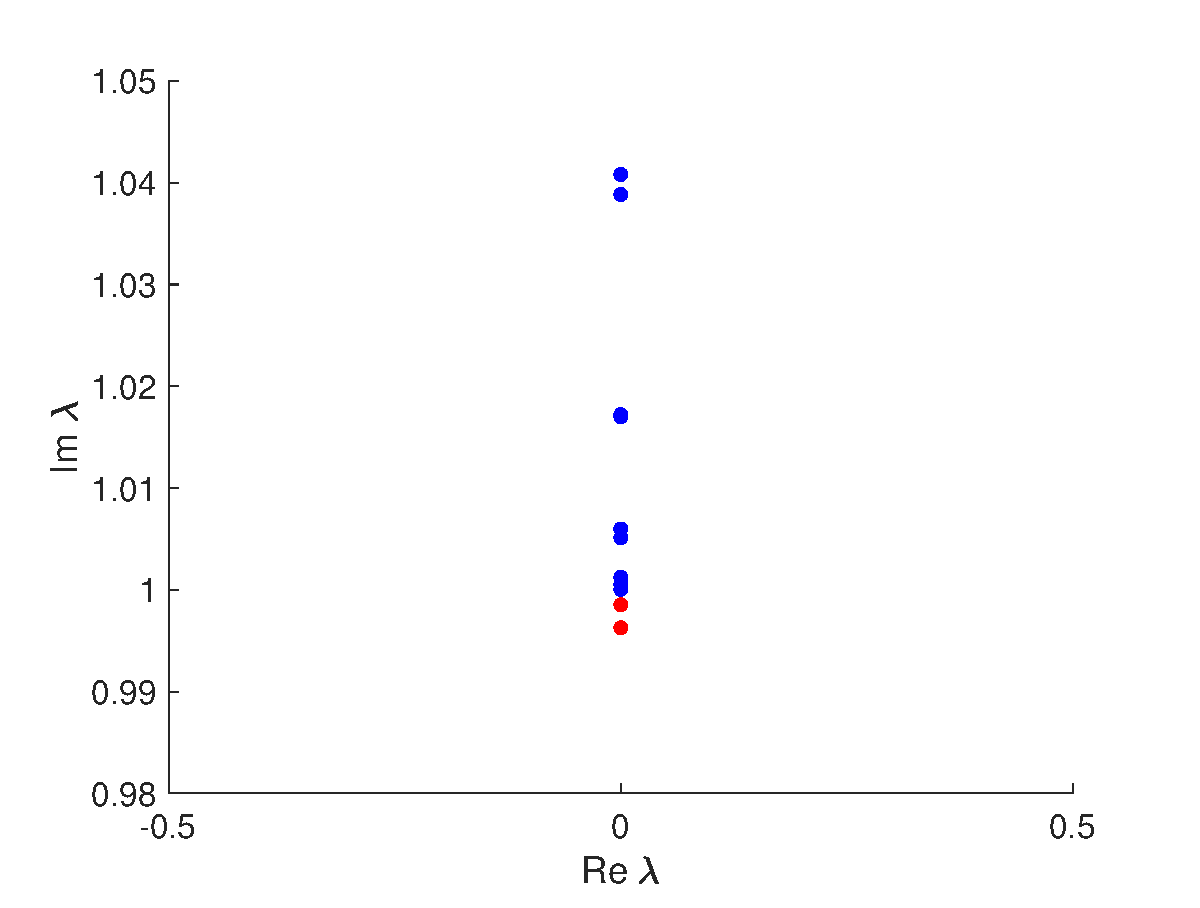
\includegraphics[width=8cm]{images/DP3internalmode.eps}
\end{tabular}
\caption{Close-up of spectrum showing pair of internal mode eigenvalues (red) and eigenvalues corresponding to the essential spectrum (blue) for third in-phase double pulse. $\beta_2 = 0$, $\beta_4 = -1$, $\omega = 1$.}
\label{fig:doubleinternalmode}
\end{figure} 

Finally, \cref{fig:inteigpred} plots the log of the relative error for the eigenvalues $\lambda_\pm$ between the value computed by Matlab's eigenvalue solver \texttt{eig} and that given by the leading order term in the formula \cref{inteigpred} versus the pulse separation distance $X$. The error decreases as $X$ increases, as predicted. The error plots are not as ``neat'' as I might like, but that is likely a result of the error in computing the terms in \cref{inteigpred}, which requires evaluating the primary pulse along an exponentially decaying tail.

\begin{figure}[H]
\centering
\begin{tabular}{c}
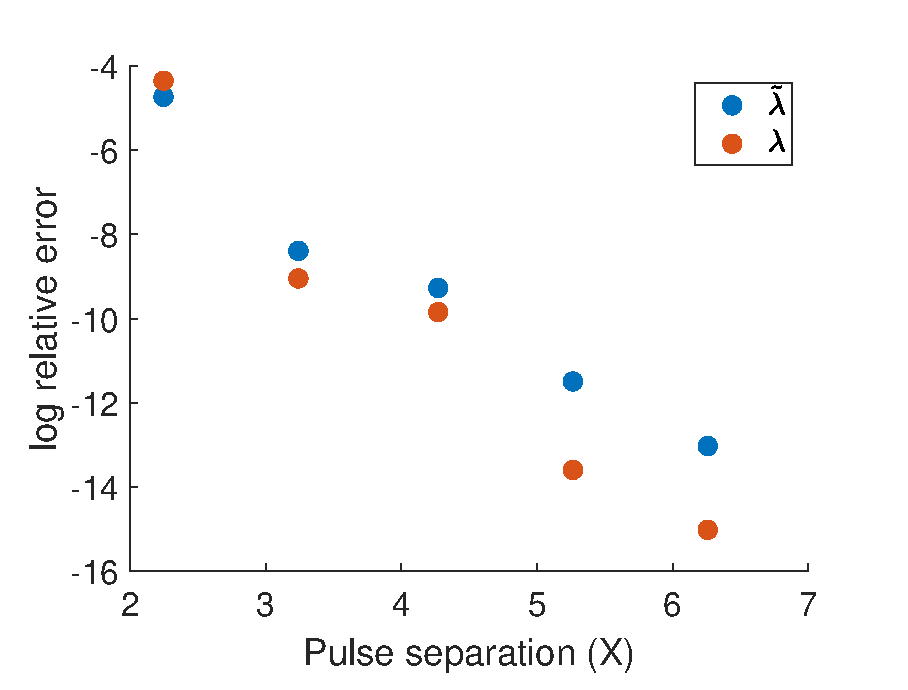
\includegraphics[width=8cm]{images/inteigpred.eps}
\end{tabular}
\caption{Log of the relative error for the eigenvalues $\lambda_\pm$ versus the pulse separation $X$ for in-phase double pulses 2-5. $\beta_2 = 0$, $\beta_4 = -1$, $\omega = 1$.}
\label{fig:inteigpred}
\end{figure}

 makes the equation for f parameter free ?

% \bibliographystyle{amsalpha}
\bibliography{NLS4.bib}

\end{document}